\chapter{Multi Type Sparse Blind Deconvolution STM (MTSBD-STM)}
\section{Challenge Formulation}
\subsection{Speckle challenge}
Speckles capture the information of the spatial distribution of defects. However, the quasiparticle band structure information is embedded in the \ac{QPI} pattern of an individual defect. Therefore, to address the challenge of speckles is to disentangle the spatial information from the \ac{QPI} pattern, and this can be formulated mathematically as a deconvolution problem. 
\par \noindent Recall that we can write the modulation of \ac{LDOS} from multiple defects as:
\begin{equation}
	\delta \rho(\mathbf{x}, \omega) = \sum_{j=1}^{N}c_j \cdot \delta \rho_0(\mathbf{x}-\mathbf{x_j},\omega),
\end{equation}
\noindent where defects are located on $\mathbf{x_j}$. We can further separate the spatial information by utilizing a Kronecker delta $\Delta(\mathbf{u})$, so that $\Delta(\mathbf{u})=1$ if $\mathbf{u} = 0$, and $\Delta(\mathbf{u})=0$ elsewhere: 
\begin{equation}
	\sum_{j=1}^{N}c_j \cdot \delta \rho_0(\mathbf{x}-\mathbf{x_j},\omega) = \sum_{\mathbf{u}} \delta \rho_0(\mathbf{x}-\mathbf{u},\omega)\cdot(\sum_{j=1}^{N} c_j \cdot \Delta(\mathbf{u-x_j})).
\end{equation}
\noindent We can then construct a convolution sum between the individual \ac{QPI} pattern and the spatial information by defining a defect location function $D(\mathbf{x}) \equiv \sum_{j=1}^{N} c_j \cdot \Delta(\mathbf{u-x_j})$, we have: 
\begin{equation}
 	\delta \rho(\mathbf{x}, \omega) =  \sum_{\mathbf{u}} \delta \rho_0(\mathbf{x}-\mathbf{u},\omega)\cdot D(\mathbf{u}) = (\delta \rho_0 *D)(\mathbf{x}, \omega).
\end{equation}

We illustrate this convolution in Fig. \ref{fig:ch6_decon}; First, we use $\delta \rho_0$ simulated in Ch.5.2 as the \ac{QPI} pattern from an single defect, we then randomly generate a binary defect location map given a defect density, and use the convolution sum to construct an observation Y. To unify the language, we will refer the single defect \ac{QPI} pattern as a kernel, denoted as A; and the defect location map as an activation map, denoted as X. Therefore, if we can successfully deconvolute A and X from Y, the challenge of speckles can be addressed.

\begin{figure}
	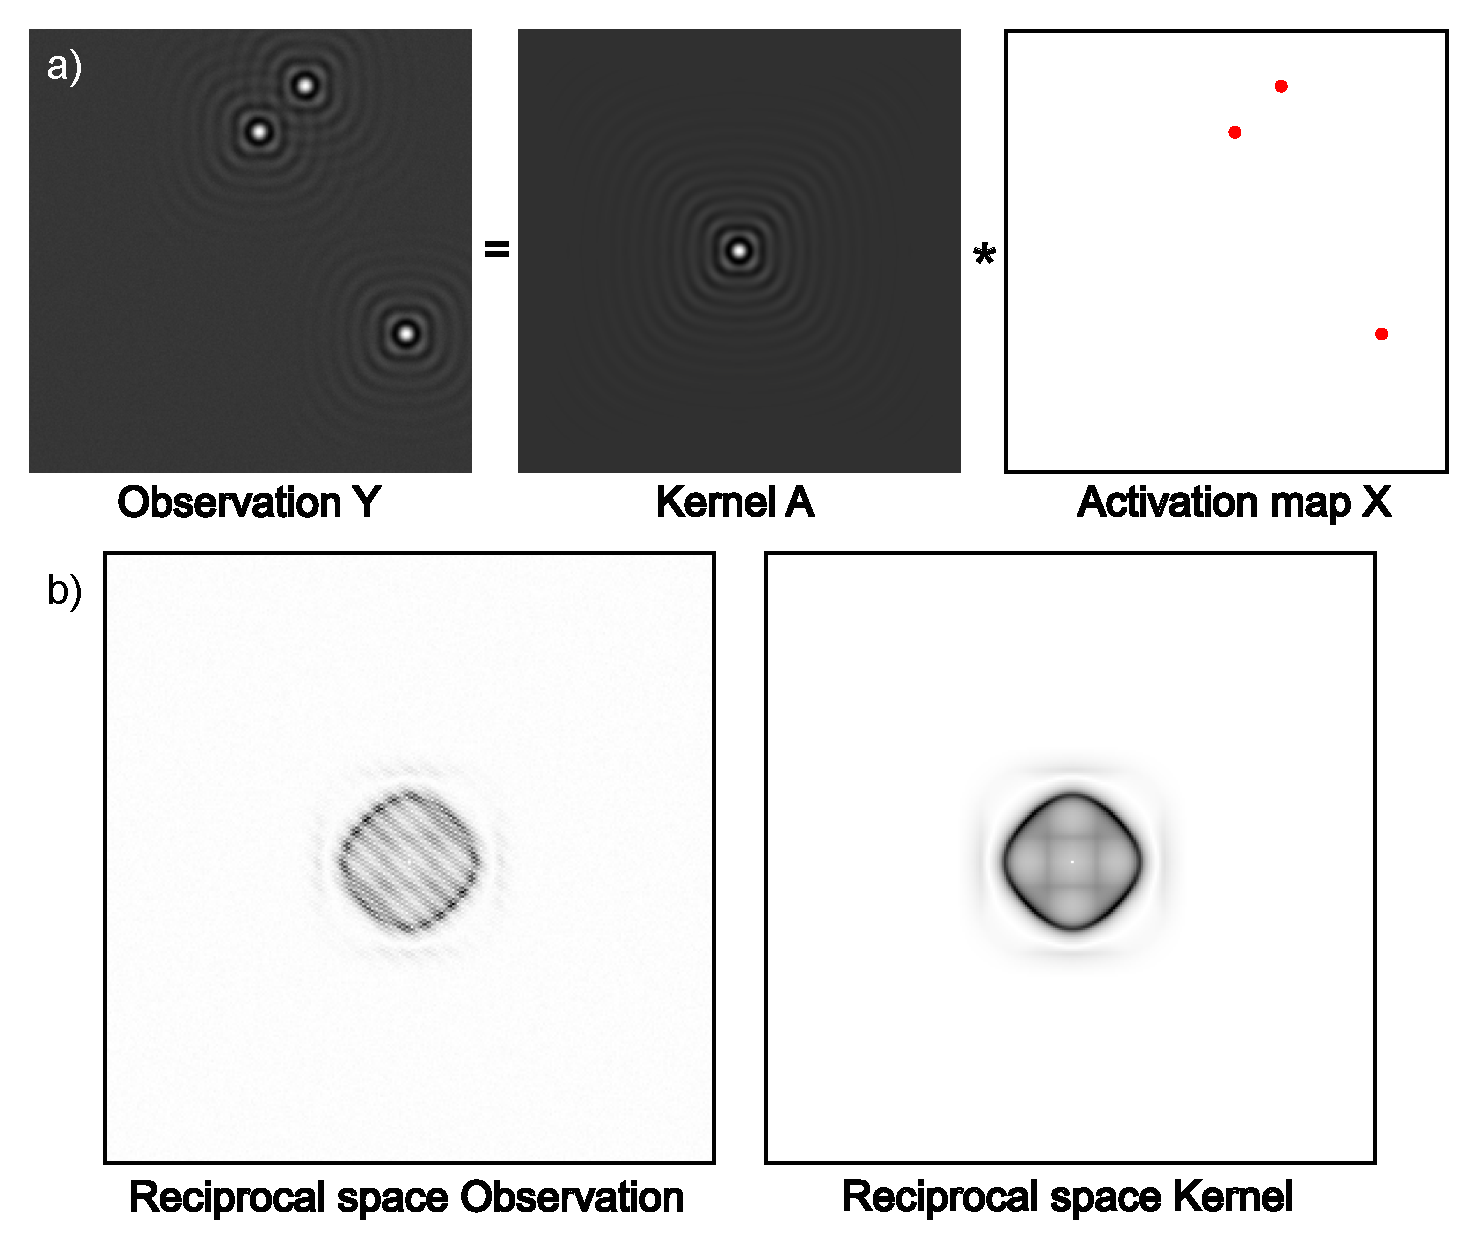
\includegraphics[width= \textwidth]{Ch6_deconvolution.pdf} 
	\centering
	\caption{}
	\label{fig:ch6_decon}
\end{figure}

\subsection{Mixing challenge}
Materials normally exhibits different types of impurities under STM, in the case of PtSn$_4$, we have 
\section{Challenges of the conventional analysis methods}
In this section, I will briefly introduce the conventional analysis methods used in the field, 2 fundamental challenges faced with the current method, and discuss the existing approaches to address these challenges and their limitations. 

Fundamentally, experimental results capture the interaction between the probe and the target; To distill the scientific essence presented in the results, complex analysis are usually required. In the case of microscopy measurements like STM, conventional methods like \ac{FT} are commonly used. %todo: add citations on examples of FT microscopy.
The \ac{FT} reveals characteristic wavelengths and provides insights to the underlying scientific theories of the specimen studied; This is particularly true in cases where the microscopy results contain near perfect periodic features, but when aperiodic signals are presented, the \ac{FT} is less ideal and suffers from loss of information. 

There are 2 specific challenges in QPI analysis with conventional \ac{FT} method we would like to focus on, the speckle problem, and the demixing problem. We will also establish their mathematical formulations, which will lead to the convolutional data model we present later. 

\subsection{The Speckle problem}
As introduced in the end of Ch5 and theorized explicitly in Equation \ref{eq.539}, when we take \ac{FT} of the grid map on multiple occurrence of defects, we get speckles on the \ac{FT-STS}; The problem is that the spatial distribution information of the defect location manifest as undesirable patterns in the \ac{FT} space, and makes the QPI pattern hard to interpret.

Therefore, to address the challenge of speckles is to disentangle the spatial information from the \ac{QPI} pattern, and this can be formulated mathematically as a deconvolution problem. 

\par \noindent Recall that we can write the modulation of \ac{LDOS} $\delta \rho$ from multiple defects as:
\begin{equation}
	\delta \rho(\mathbf{x}, \omega) = \sum_{j=1}^{N}c_j \cdot \delta \rho_0(\mathbf{x}-\mathbf{x_j},\omega),
\end{equation}
\noindent where $\delta \rho_0$ is the \ac{LDOS} modulation from individual defect located at at $\mathbf{x_j}$. We can further separate the spatial information by utilizing a Kronecker delta $\Delta(\mathbf{u})$, so that $\Delta(\mathbf{u})=1$ if $\mathbf{u} = 0$, and $\Delta(\mathbf{u})=0$ elsewhere: 
\begin{equation}
	\sum_{j=1}^{N}c_j \cdot \delta \rho_0(\mathbf{x}-\mathbf{x_j},\omega) = \sum_{\mathbf{u}} \delta \rho_0(\mathbf{x}-\mathbf{u},\omega)\cdot(\sum_{j=1}^{N} c_j \cdot \Delta(\mathbf{u-x_j})).
\end{equation}
\noindent We can then construct a convolution sum between the individual \ac{QPI} pattern and the spatial information by defining a defect location function $D(\mathbf{x}) \equiv \sum_{j=1}^{N} c_j \cdot \Delta(\mathbf{u-x_j})$, we have: 
\begin{equation}
	\delta \rho(\mathbf{x}, \omega) =  \sum_{\mathbf{u}} \delta \rho_0(\mathbf{x}-\mathbf{u},\omega)\cdot D(\mathbf{u}) = (\delta \rho_0 *D)(\mathbf{x}, \omega).
\end{equation}

We illustrate this convolution in Fig. \ref{fig:ch6_decon}; First, we use $\delta \rho_0$ simulated in Ch.5.2 as the \ac{QPI} pattern from an single defect, we then randomly generate a binary defect location map given a defect density, and use the convolution sum to construct an observation Y. To unify the language, we will refer the single defect \ac{QPI} pattern as a kernel, denoted as A; and the defect location map as an activation map, denoted as X. Therefore, our goal is that given $Y = A * X$, we want to reconstruct A and X. 

\begin{figure}
	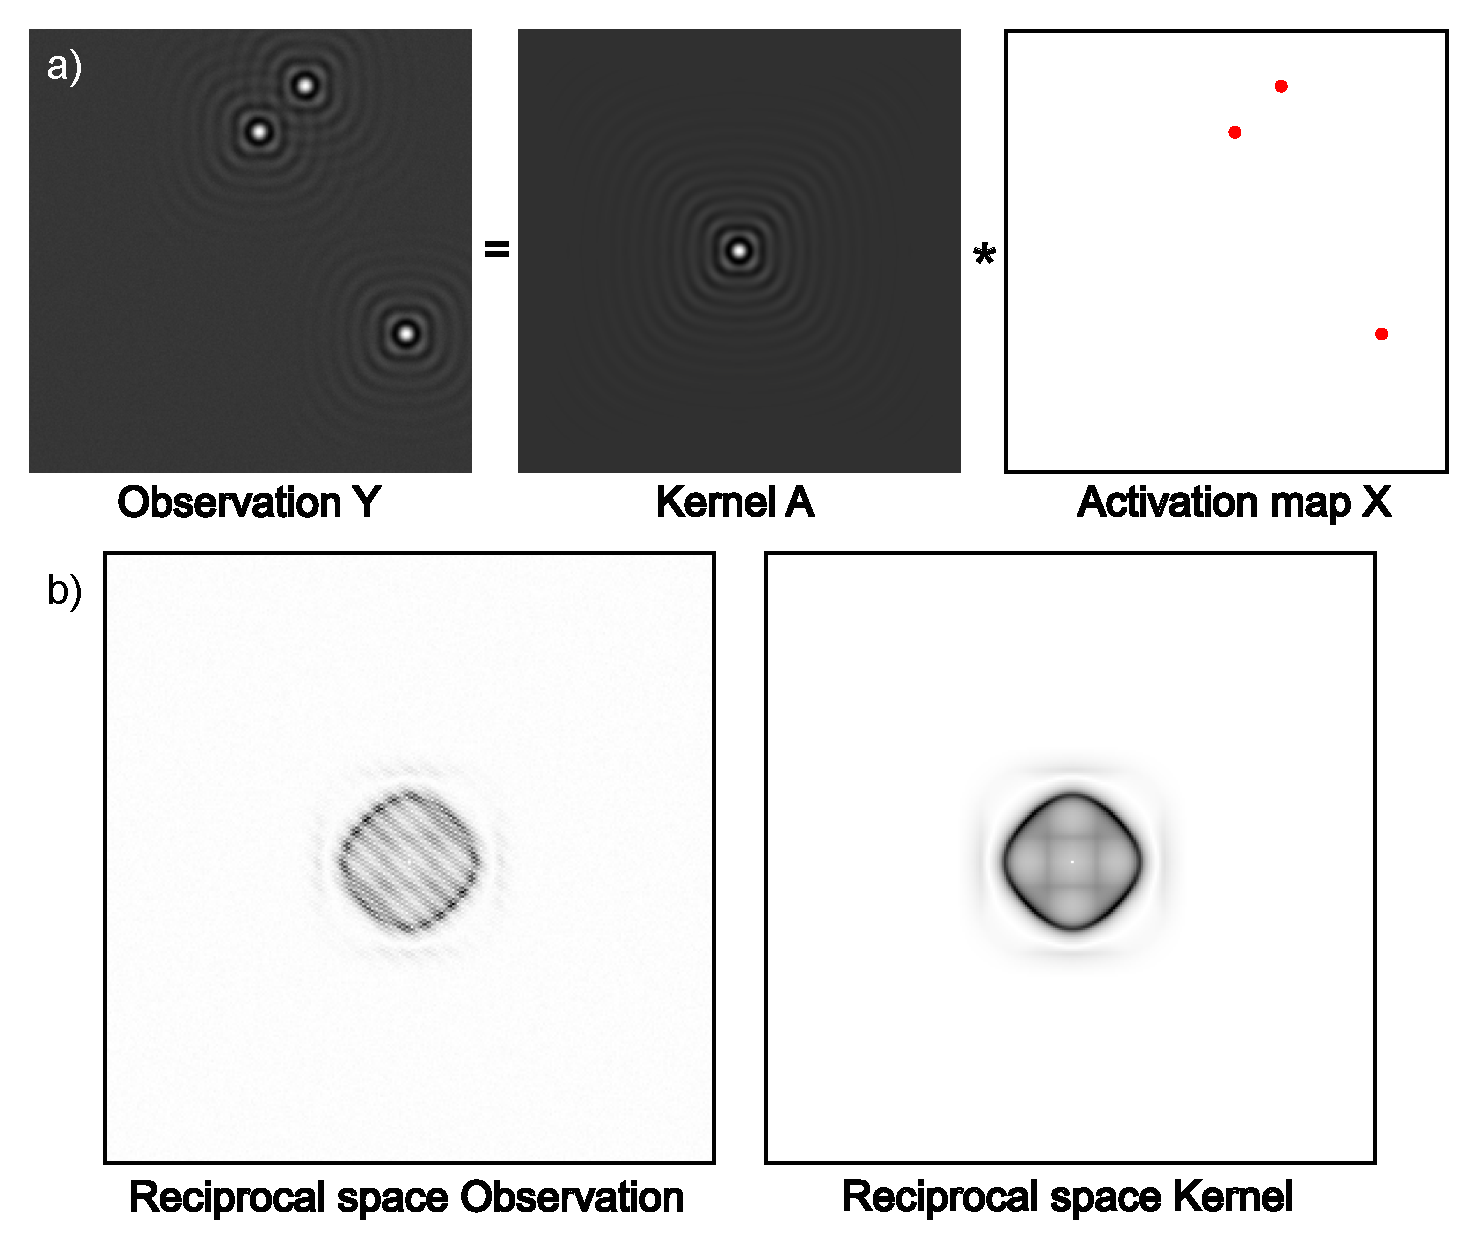
\includegraphics[width= \textwidth]{Ch6_deconvolution.pdf} 
	\centering
	\caption{}
	\label{fig:ch6_decon}
\end{figure}

\subsection{The Demixing problem}
%todo: how should I include the general motivation of demxing? or is it enough here? 
Materials normally exhibit multiple types of defects, and these defects can present different scattering features; Many QPI measurements have exploited the mechanisms of selectivity scattering channels across a wide variety of materials, such as the sign variation of the superconducting order parameter, the spin and orbital texture of topological bands, etc. However, there are only limited approaches to analyze and disentangle defect dependent scattering features. The most common approach is to acquire grid spectroscopy on isolated defects, or to crop around individual defect in larger grid maps if isolated defect is hard to find. One example is the Dirac semimetal ZrSiS, where the interference patterns around impurities located on the Zr and S sublattice sites scatter differently \cite{butler et al}; As shown in \ref{fig:ch6_ZrSiS}, conventional \ac{FT} display a mixture of the scattering features, which are disentangled through inspecting the \ac{FT} of cropped grid spectroscopy around individual defects. 

There are 2 primary shortcomings with this approach, one is due to small spatial range of the cropping, the resolution in q-space is very much limited, making it hard to resolve features with higher frequencies. Second is that the cropped area could still preserve features from other defect sources, this is particularly problematic when we have quasiparticles with longer lifetime; The long decaying tail could easily spread tens or hundreds of unit cells, making it hard to avoid when cropping. 

\begin{figure}
	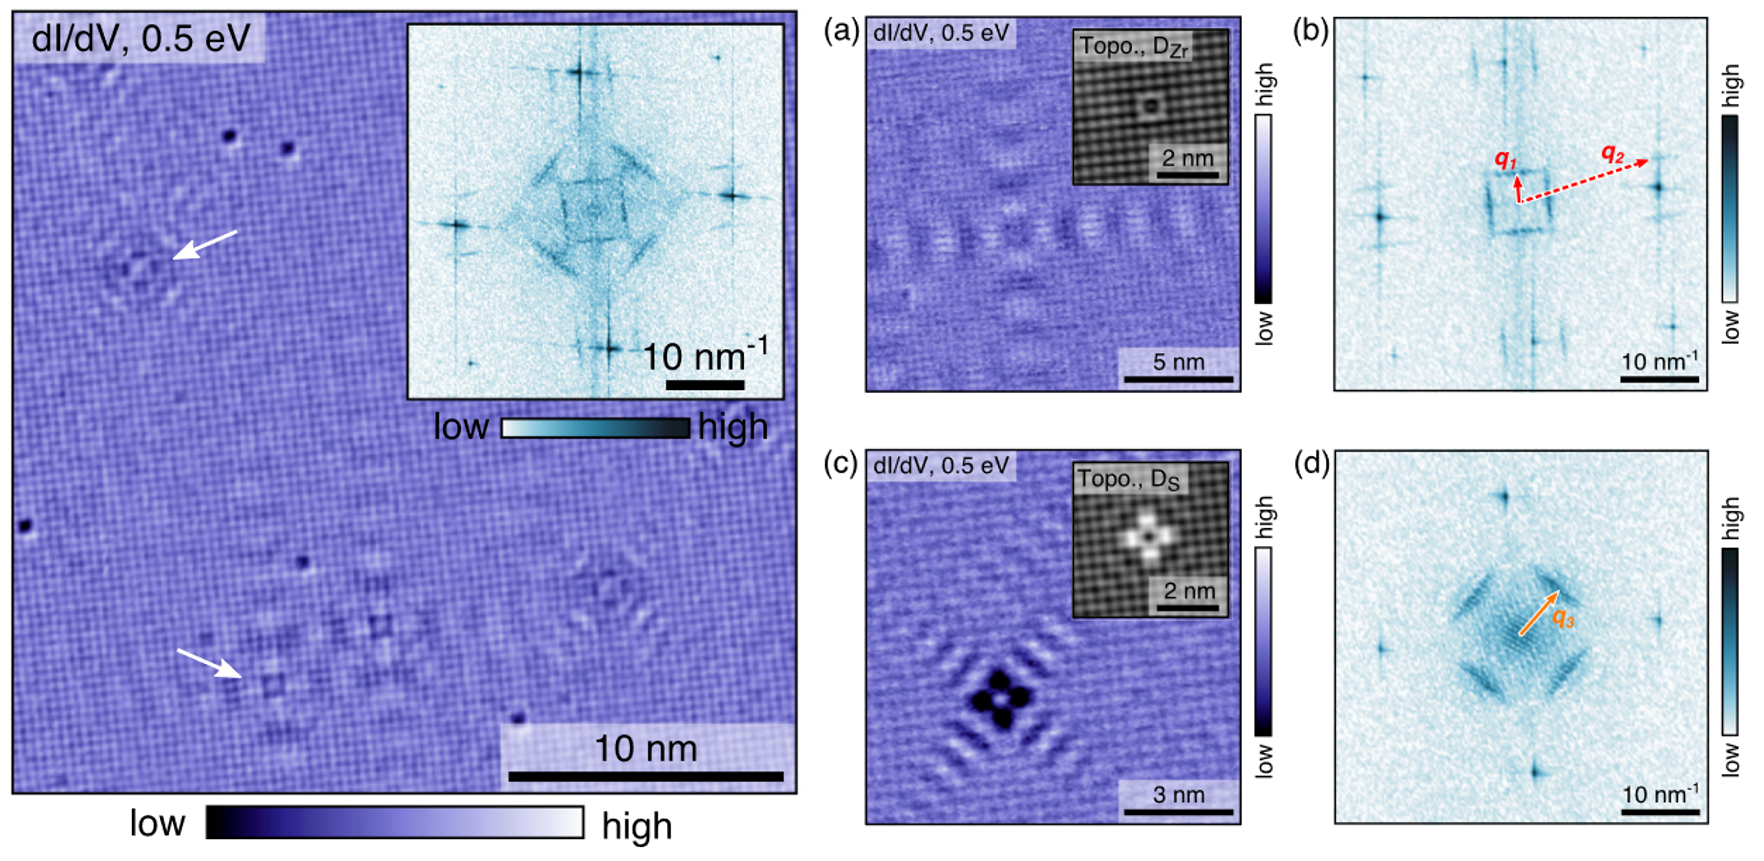
\includegraphics[width= \textwidth]{ZrSiS.png} 
	\centering
	\caption{}
	\label{fig:ch6_ZrSiS}
\end{figure}
%todo: add citations to corresponding literatures 

It is therefore preferred, if we can reconstruct the contribution of each individual type of defect from a big grid map that includes multiple types of defects; this is called the demixing problem.  

We now use our synthetic data to better illustrate the demixing problem. We simulate 2 \ac{QPI} patterns from 2 distinct defects with kernel choices A1 and A2 as shown in Fig. \ref{fig:ch6_demix} c) and d); We then define their activation maps X1 and X2 in d) and g). By summing up the convolutions between 2 kernels and their corresponding activation maps, we can obtain an observation Y in a). We express the above observation generation process as:

\begin{equation}
	Y = A1 * X1 + A2 * X2 + \beta, 
\end{equation}
where $\beta$ is the added noise determined by a pre-defined signal-to-noise ratio.

The demixing problem is the inverse of the observation generation process: given the observation 
Y, our goal is to reconstruct A1, A2, and their corresponding activation maps. This means that in reciprocal space, rather than working with entangled and less informative data like (b), we can recover disentangled QPI patterns from individual defect types, as shown in (e) and (h), which are also free from speckles. Lastly, we extend the above formulation with multiple types of different defects, then at arbitrary energy $\omega$, we have: 

\begin{equation}
	\label{eq:demixing}
	Y_{\omega} = \sum_d ( A_{d,{\omega}} * X_d) + \beta. 
\end{equation} 

\begin{figure}
	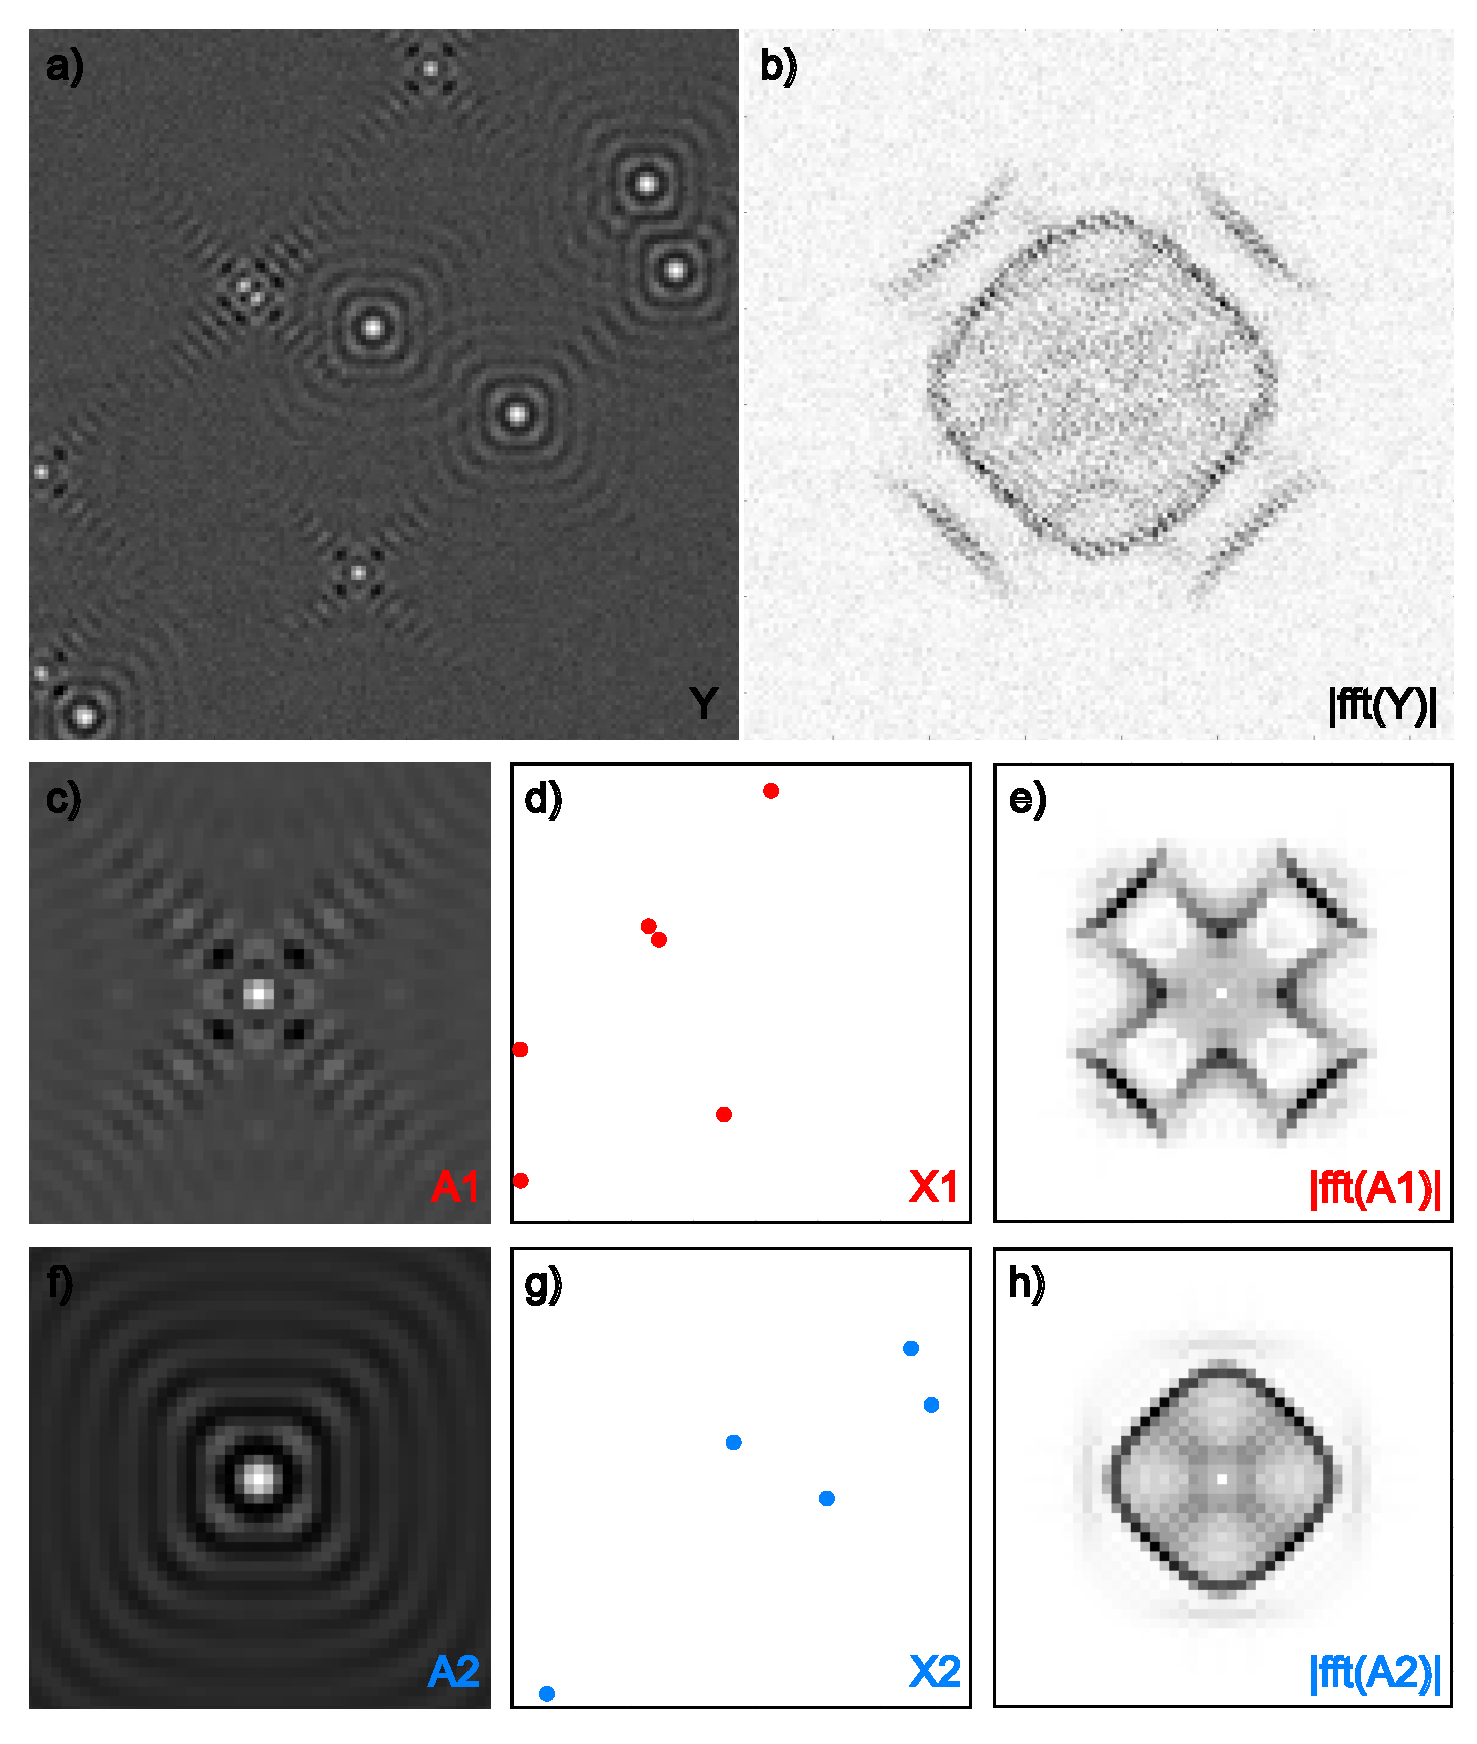
\includegraphics[width= \textwidth]{Ch6_demixing.pdf} 
	\centering
	\caption{}
	\label{fig:ch6_demix}
\end{figure}




\section{Existing Algorithm}
\subsection{Shortcomings of existing algorithm}
\begin{itemize}
	\item 1. Their simulation data used truncated QPI pattern, not true to the real STM case. 
	\item 2. Too ideal to be useful in most cases,
\end{itemize}

Shortcoming in generating the observations. The purpose here is to simulate as close to experiment as possible to test and benchmark this method. 

I would like to elaborate on the truncation they made, they are given a simulation result, say a $256\times256\times41$ of $\delta\rho$ covering say 50 by 50 lattice from single defect at the center, without considering the noise level, the authors truncate the initial 50 by 50 lattice down to 19 by 19. In the generation of the observation, a parameter is set to be the ratio between the kernel size versus the window size, by setting this, they determined target size of the kernel in pixel, and then they can reshape the 19 by 19 lattice simulation into the target size. While one can argue that this process of truncating and reshape did not hinder the purpose of testing the SBD algorithm. It fails to simulate what happened in the experiment. Note that with this method, the boundary of the real-space QPI pattern is artificially set by the truncation.

Physically, the boundary of real-space QPI pattern is resulted from the interplay between the quasiparticle lifetime and the noise level, as kind of illustrated in Fig. \ref{fig:ch5_cutoff}; Thus, the kernel-window size ratio can be calculated after setting up the designed noise level at an energy slice, and due to this direct correlation, we argue that this is not a well-defined free parameter to be considered in the simulation. 

The way they simulate the observation is through the 2D convolution between a reshaped kernel with QPI pattern and an ideally binary activation; The convolution thus enforced defects sitting at activation pixels with entry equal to one. As defects can only site on the lattice sites, this only make sense when we define the activation map as the lattice site, which is not how it is defined in this work. 

The conflict here is that we need 2 uncorrelated free parameters to define the spatial unit of the observation. one is the number of lattice sites contained in the observation, the second is the spatial resolution of the observation. The former determines the spatial range of this observation, and the latter determines the physical separation between adjacent pixels. 
 
 
\subsection{Our mitigation}

We can thus propose a more physical way to simulate the observation, as follows: 
For a synthetic observation $Y(\omega)$ at energy $E=\omega$, we first take the single defect QPI simulation $\delta\rho_{single} (\omega)$ at that energy, choose an SNR-ratio $SNR$ and apply it onto $\delta\rho_{single} (\omega)$, we can then draw an cutoff location where the signals are buried in the noise, this cutoff location is defined both at the pixel location and the lattice location of $\delta\rho_{single} (\omega)$. Then we choose N that defines the observation on an $N\times N$ lattice sites, and we can choose a linear resolution $\lambda = 1/p$ per lattice site, where $p$ is an integer, this then gives us a $pN \times pN$ pixel observation.
We then define an activation map X that is $N\times N$, then we choose a surface defect density $\rho_d$ and randomly assign the number of defects onto the X, we then can then match the dimension of X with Y, through an upsampling function that takes a matrix and expands it by a specified scale factor by placing each original value in a grid of zeros, effectively creating a larger sparse matrix where original values are separated by zeros in both horizontal and vertical directions. More specifically, we want to upsample X by $p$ to get dimension of $pN \times pN$. 
Recall that we have the $\delta\rho_{single} (\omega)$ cutoff at a certain lattice site M and corresponding pixel, now before we perform the convolution, we need to unify the spatial representation of the $\delta\rho_{single} (\omega)$ and Y, more specifically, we need to resize the $\delta\rho^{cutoff}_{single} (\omega)$ to match the pixel size in the observation corresponding to M lattice sites. that is $\delta\rho^{resized}_{single}= imresize(\delta\rho^{cutoff}_{single} (\omega)$, [pM, pM]). And then Y= convolution($\delta\rho^{resized}_{single} (\omega)$, $X^{upsampled}$)

To avoid truncated QPI pattern, during simulation. There are a few things to keep in mind: 
\begin{itemize}
	\item 1. Forming observation by 2d convolution of activation and single defect QPI pattern is much time/computationally efficient to work with, than directly simulate multi defect QPI pattern. 
	\item 2. So we will use single defect QPI pattern. 
	\item 3. To simulate single defect QPI pattern, we will need to define, apart from the lattice constants($a$), n$_l$: number of lattice points along one dimension, and n$_p$: number of pixels of this simulation in one dimension. We can then compute the grid resolution pixel/nm that this simulation correspond to in a physical system, for instance given a lattice parameter $a$, then for our kernel, we have grid resolution = $a$*n$_l$/n$_p$ nm/pixel.
	\item 4. Note that a physical activation is nothing but a r*r square lattice span some real space area of $(r*a)^2$with N$_d$ number of defect located on some of the lattice points. However, in simulation activation, we have a matrix of n*n that on each point there is a certain probability it is a defect site, this means, here n has the same physical meaning as r.
	\item 5. $Y=conv2d(X,A)$ but this convolution assumes that we have the kernel's resolution same as the activation. To make that assumption hold, we need the activation's resolution = lattice constant/pixel = a nm/pixel, then we need to have n$_l$ = n$_p$. However, this case we lost the flexibility of changing our activation resolution. Another case is to let the activation holds the same resolution to the kernel, which is conventionally arbitrary, and this is also problematic as this case we are allowing defects sitting not on their lattice site, which is only true for defects like interstitial.
	\item The ideal case would be, the  activation resolution/kernel resolution is an integer, meaning n$_l$/n$_p$ =q, q is an integer. Then we should have a fake activation whose side = n*q, where as defects are only allowed to sit in the real activation whose side is n.
\end{itemize}
Then how do we determine the window size?  
\section{SBD-STM Performance Analysis}

\section{Multi-Type-Scatters (MT) SBD-STM}


\subsection{Bench Mark of MT-SBD-STM}

\subsubsection{system parameter space}

\subsubsection{data set parameter space}